\section{AI-Assisted Authoring Workflow}
\label{sec:authoring-workflow}

Figure~\ref{fig:overall-architecture} shows the system architecture and an example flow.
The system is composed of two agents:

\begin{itemize}
    \item \textbf{SuggestionAgent}. Based on an LLM, the SuggestionAgent receives as input the initial text and the reference data, and returns the elements in the text that can be replaced with expressions in the Fluid language.
    \item \textbf{InterpretationAgent}. Also based on an LLM, the InterpretationAgent receives as input a selection (either obtained from the SuggestionAgent or manually defined by the author) and generates an interpretation of the text as a Fluid expression.
\end{itemize}

\begin{figure}
    \centering
    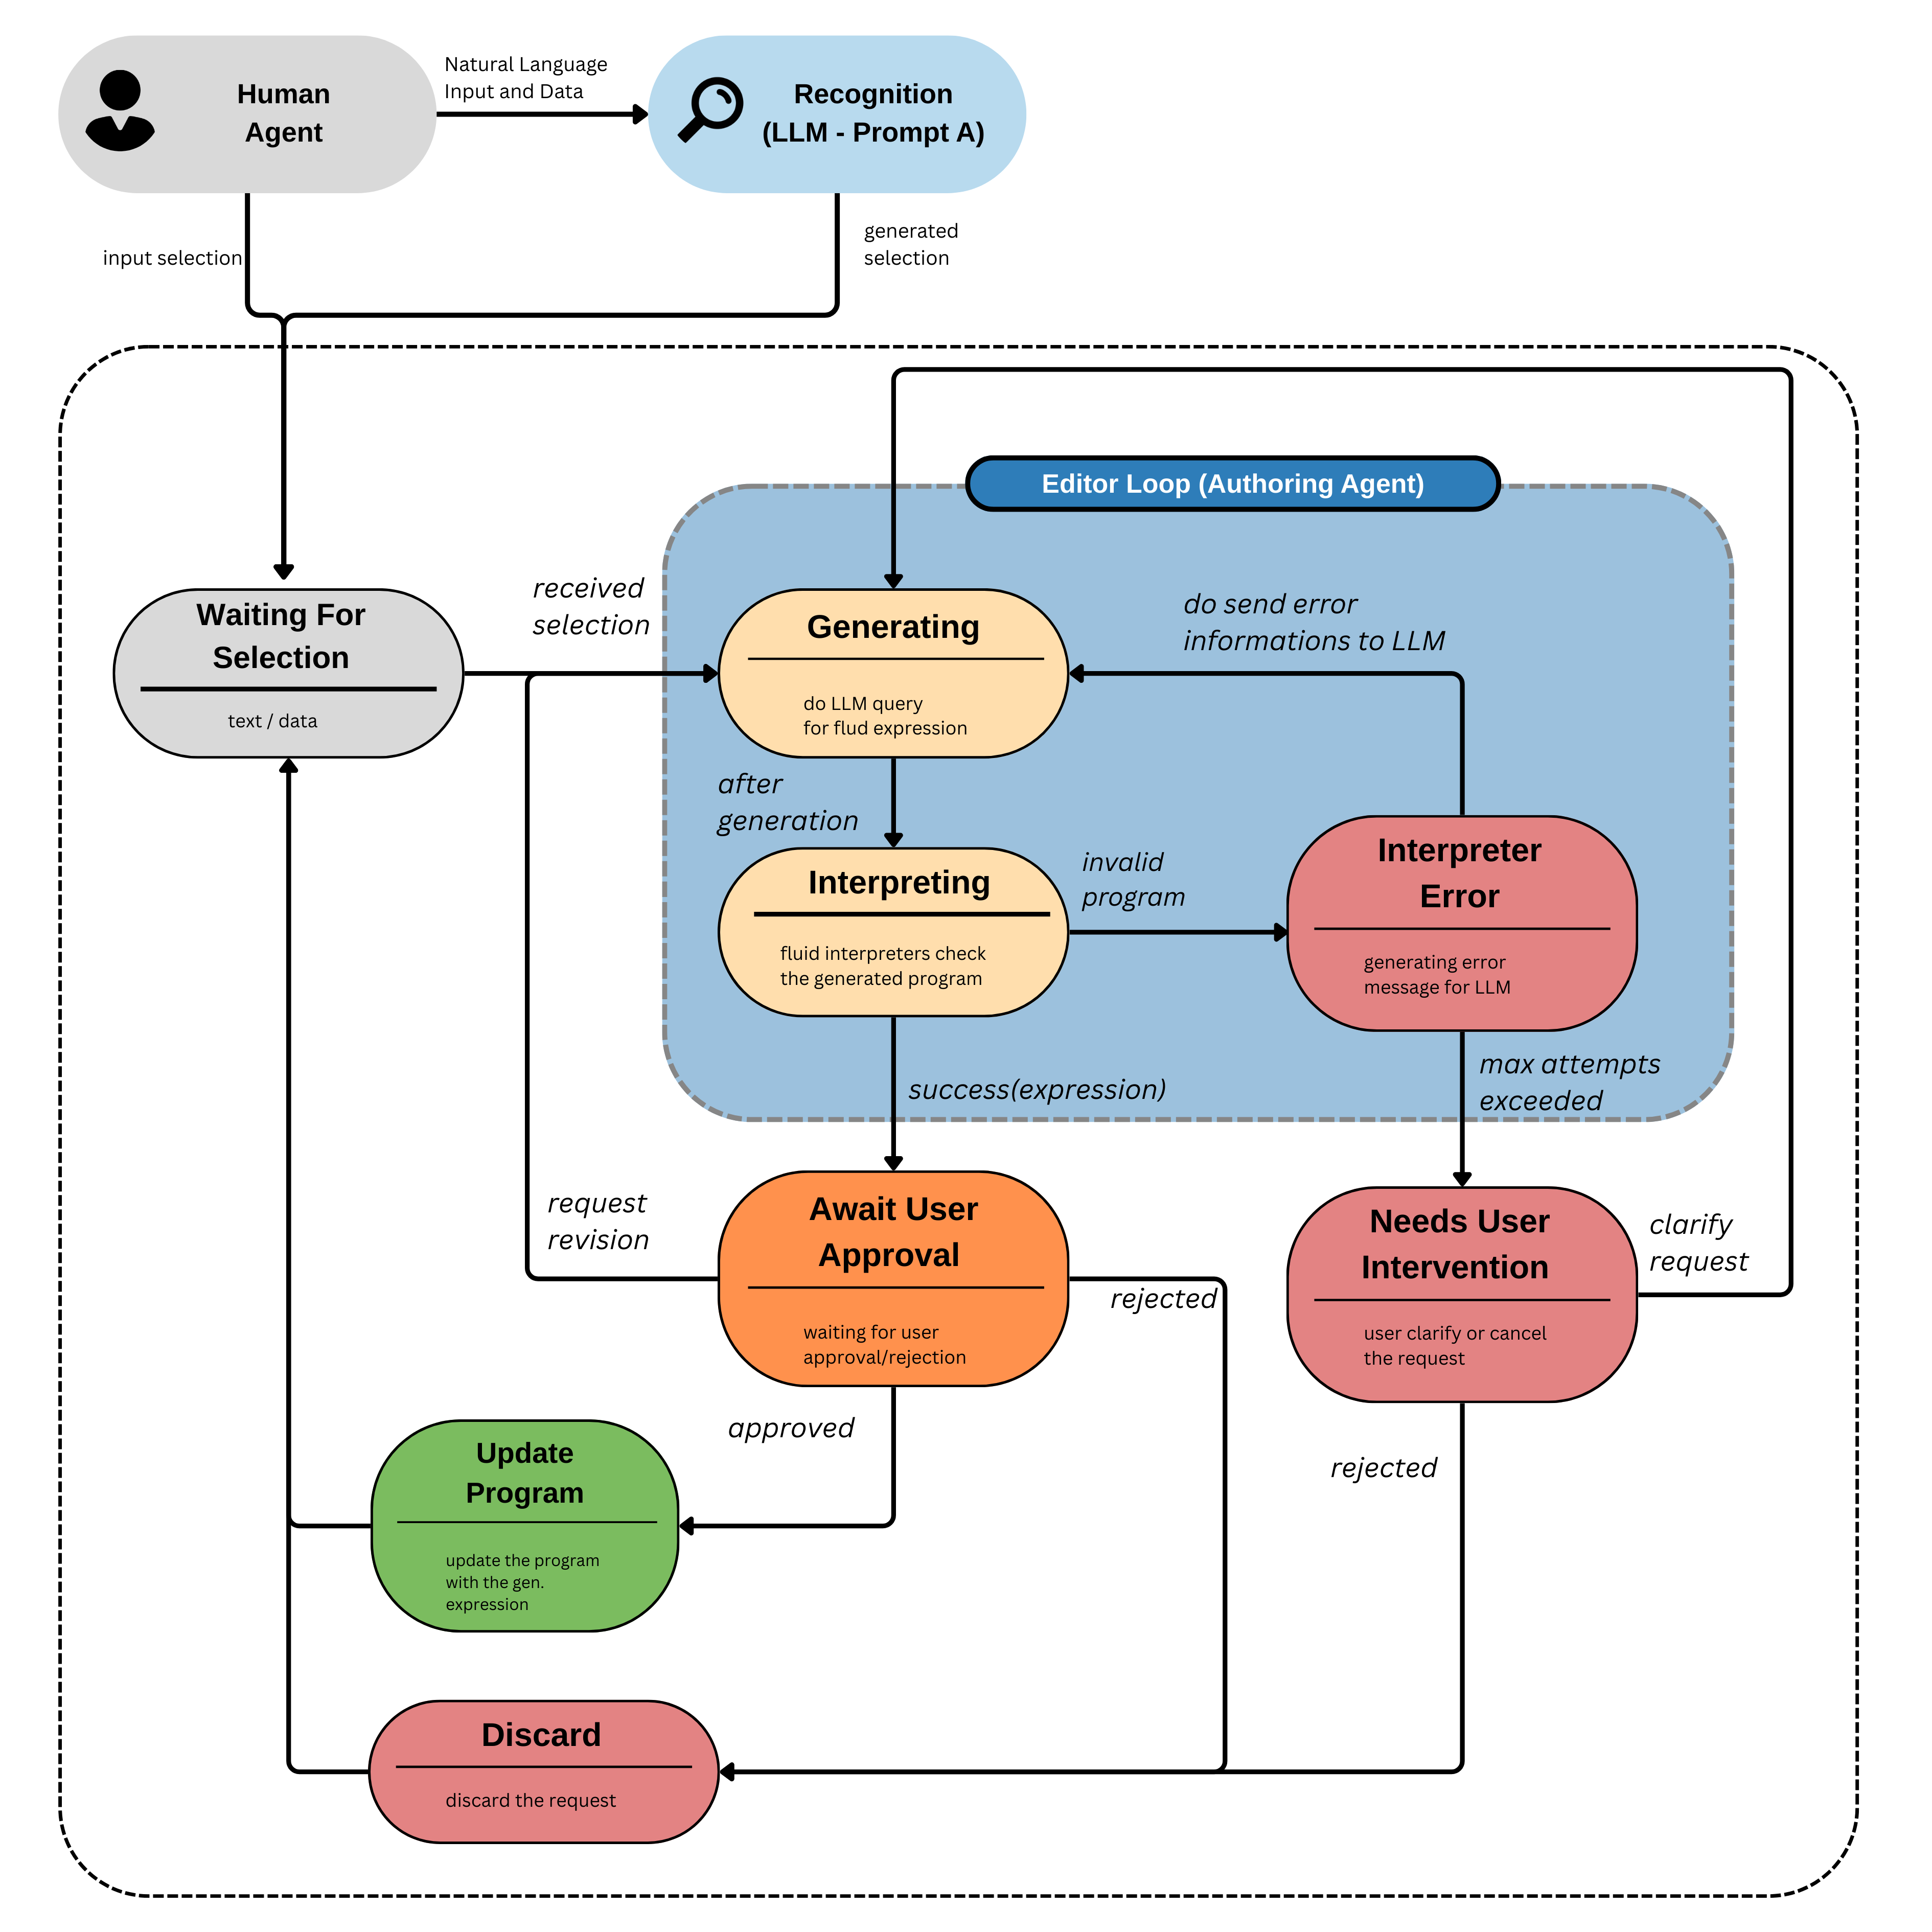
\includegraphics[width=\linewidth]{fig/entire-workflow}
    \caption{Workflow}\label{fig:architecture}
\end{figure}

Figure~\ref{fig:architecture} shows the overall architecture of the system.
The author initially provides the text and accompanying data.
The SuggestionAgent analyses the input and identifies candidate fragments of natural language which could be replaced by Fluid expressions.
The user highlightes a fragment of interest, which is then sent to the InterpretationAgent, which generates a corresponding candidate expression.
Internally the InterpretationAgent uses a compiler-in-the-loop validation process to ensure the expression is well-formed.
The user is then able to accept the expression (in which case it is incorporated into the program) or reject and leave the text uninterpreted.

\begin{figure}[ht]
    \centering
    \begin{subfigure}{0.50\linewidth}
        \centering
        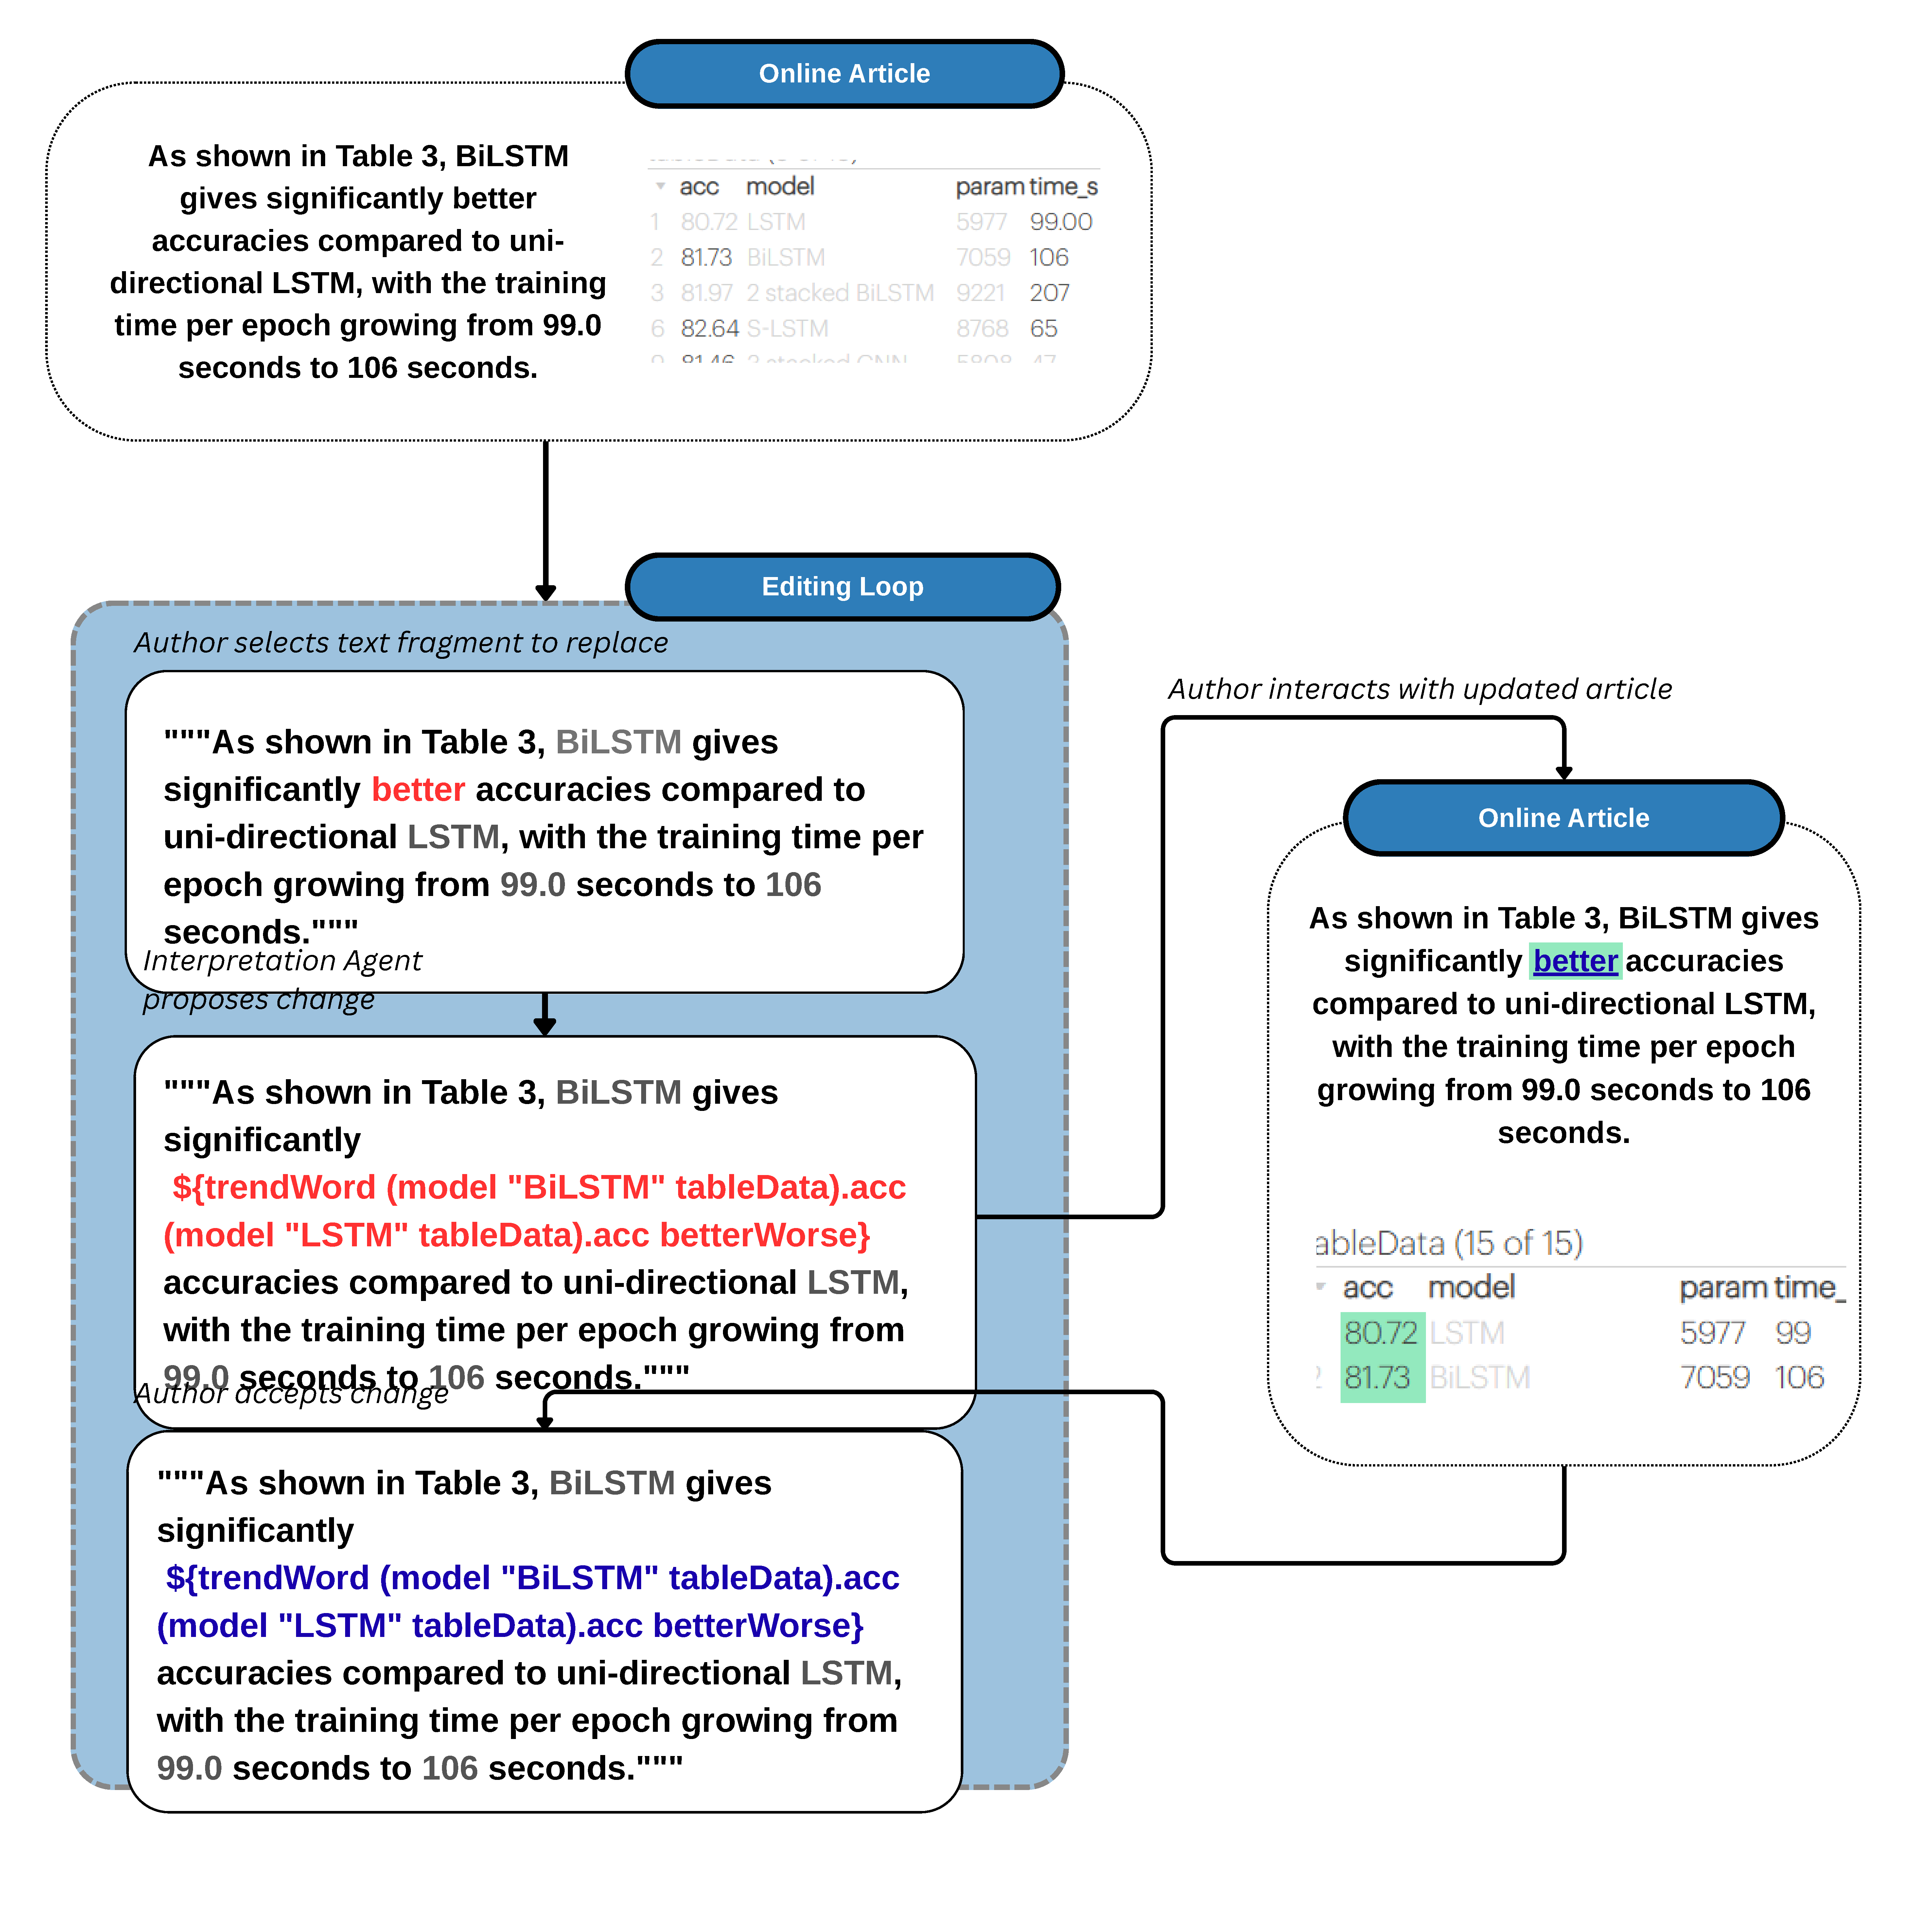
\includegraphics[width=\linewidth]{fig/data-flow-correct}
        \caption{Author Acceptance Dataflow}
        \label{fig:data-flow-correct}
    \end{subfigure}\hfill
    \begin{subfigure}{0.50\linewidth}
        \centering
        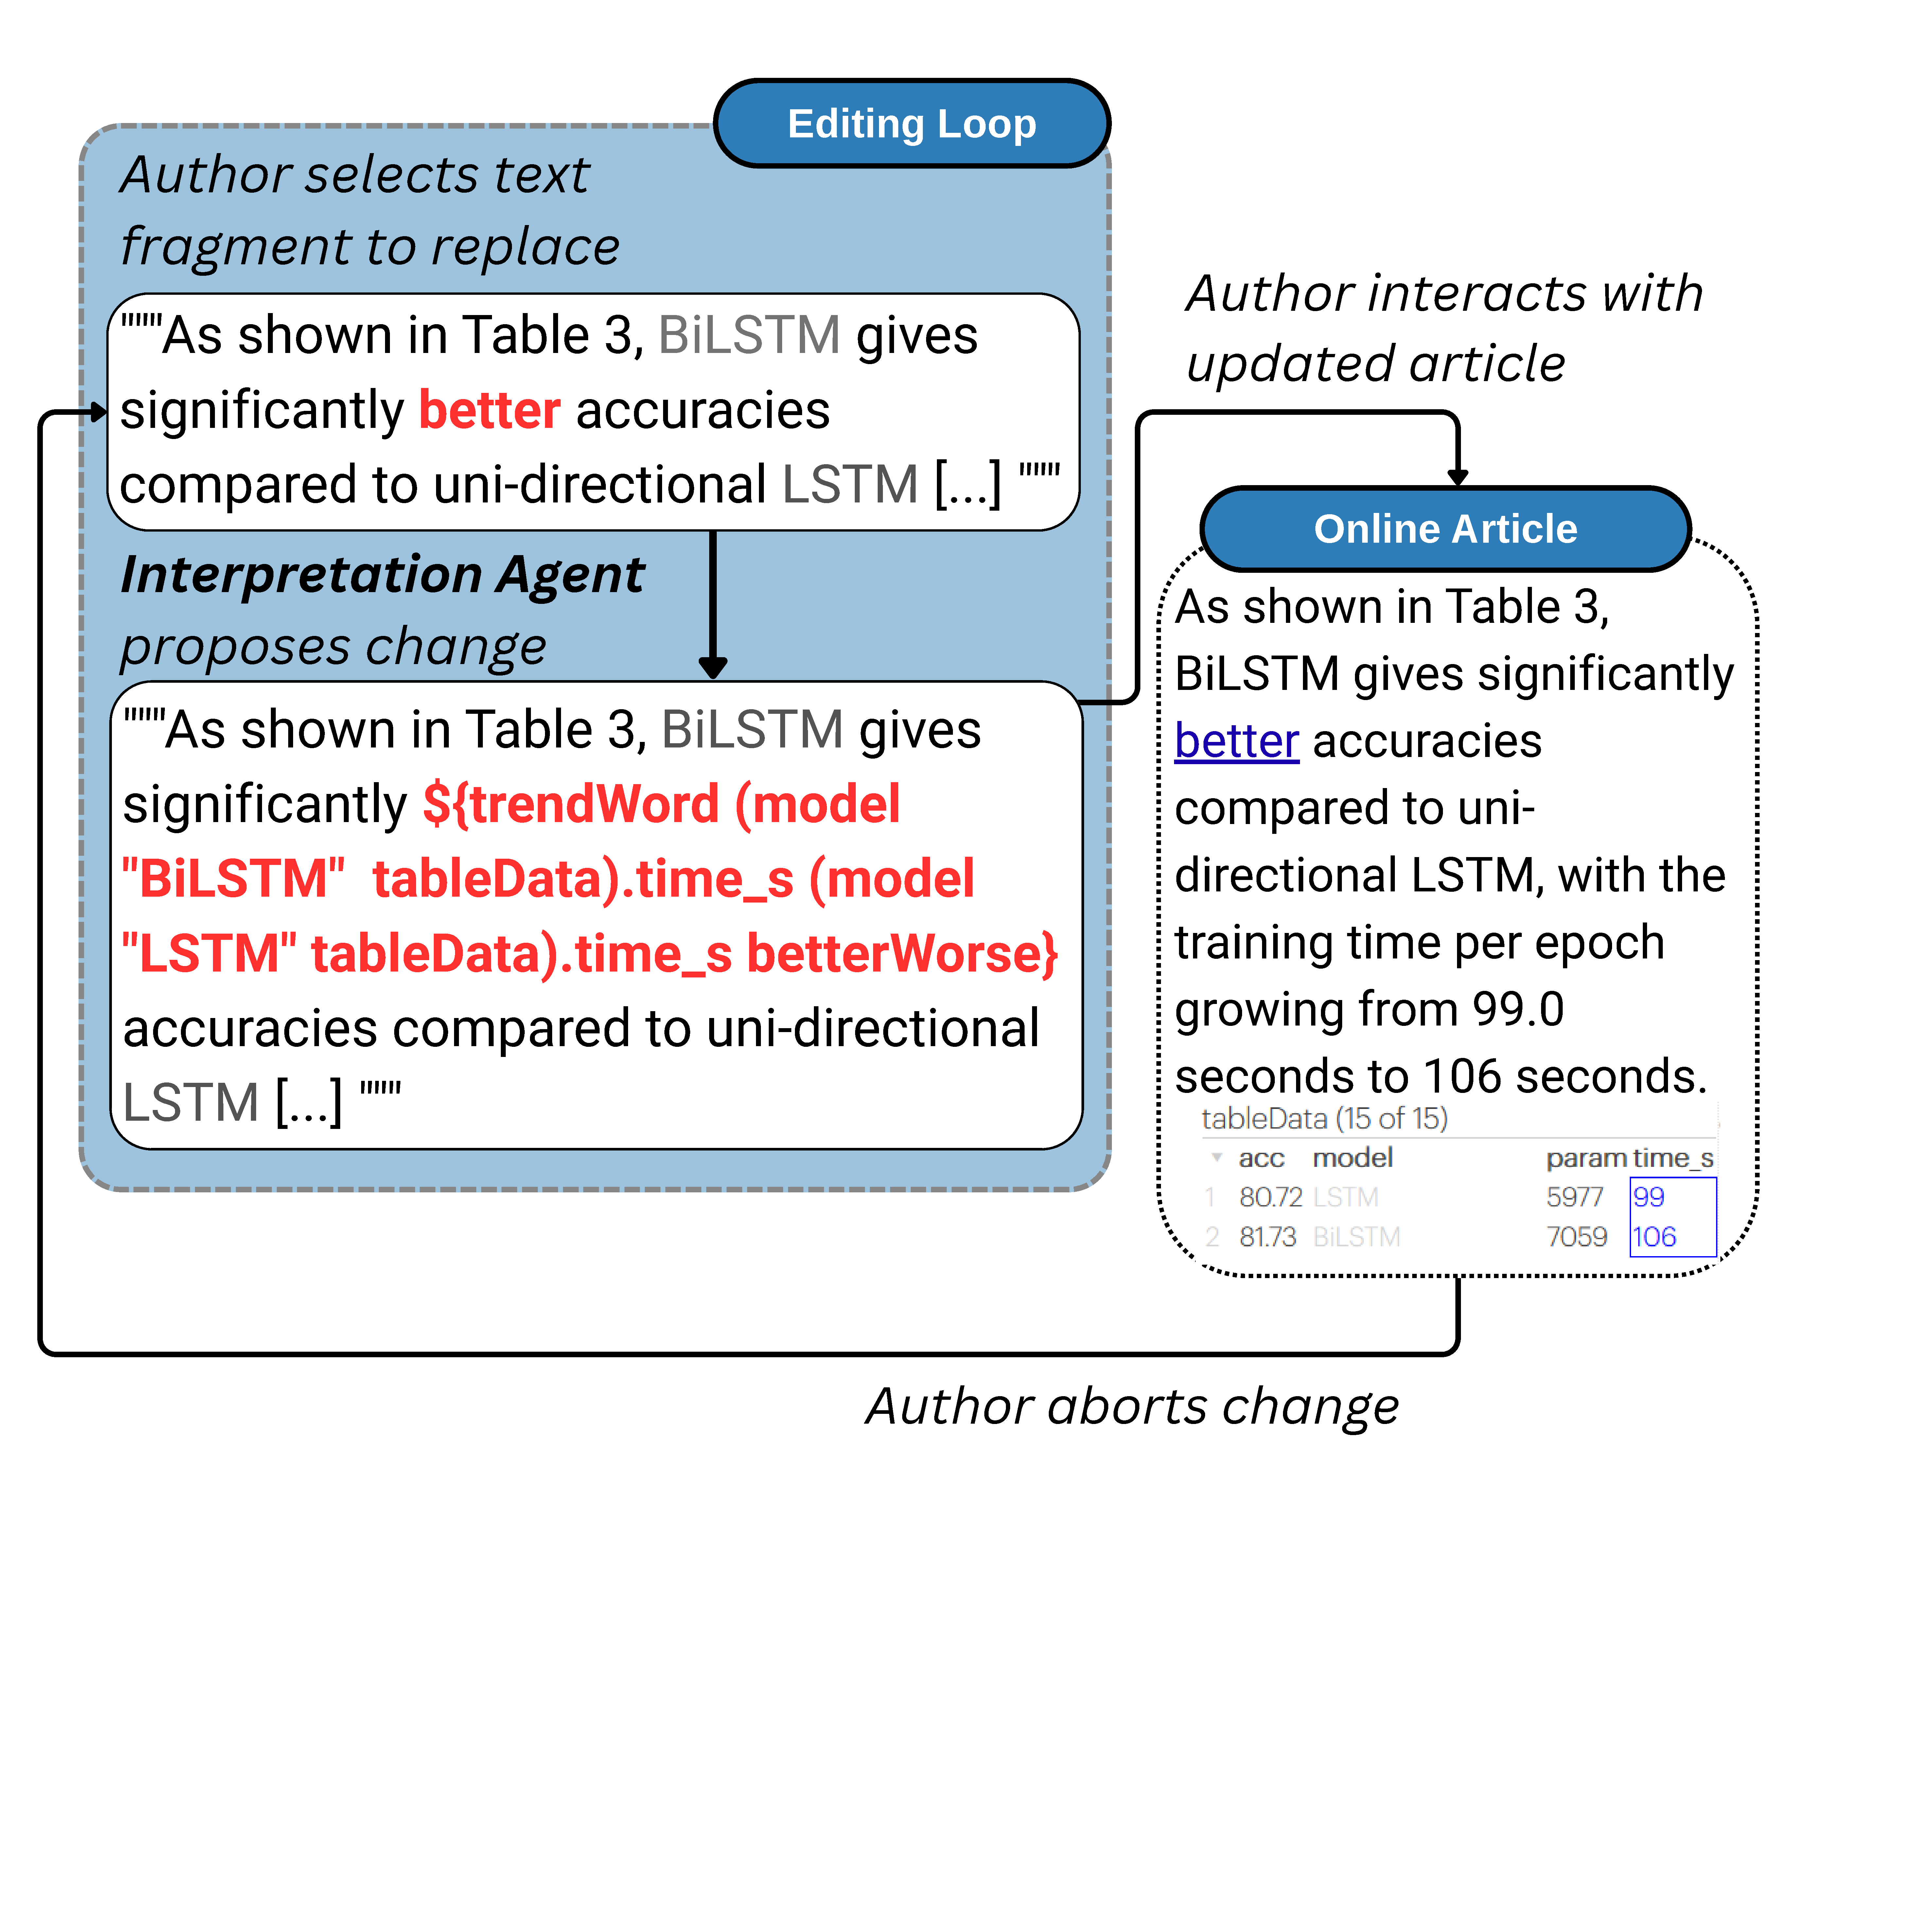
\includegraphics[width=\linewidth]{fig/data-flow-error}
        \caption{Author Rejection Dataflow}
        \label{fig:dataflow-error}
    \end{subfigure}
    \caption{Two workflows of the Interpretation Agent. In Fig. \ref{fig:data-flow-correct}, the author accepts the generated expression after verifying its correctness online. In Fig. \ref{fig:dataflow-error}, the author identifies an error (the expression mentions accuracy, while the article highlights timing) and rejects it.}
    \label{fig:overall-architecture}
\end{figure}


\subsection{System Prompt}
\label{subsec:system-prompt}
Fig. \ref{fig:system-prompt} shows the system prompt defined for the Authoring Assistant.

\begin{figure}[h]
    \centering
    \begin{tcolorbox}[colback=gray!10, colframe=gray!50, boxrule=0.5pt, arc=2pt,
        left=6pt, right=6pt, top=4pt, bottom=4pt]
        \VerbatimInput[fontsize=\small, formatcom=\normalfont]{../system-prompt/system-prompt.txt}
    \end{tcolorbox}
    \vspace{-0.5em}
    \caption{System-Prompt defined for the Authoring Assistant}
    \label{fig:system-prompt}
\end{figure}


\subsection{Editor Loop}
\label{subsec:editor-loop}
Design of main loop that would be integrated into an IDE. The configuration (state) that is being maintained
is a \kw{Paragraph} the user is authoring in Fluid. Consists of a sequence of text fragments, some of which
are uninterpreted (plain literals), the remainder have underlying expressions linking the text to raw or derived
data.

Workflow:
\begin{enumerate}
\item User selects (a substring of) one of the literal text fragments, indicating they want to link it in this
way
\item Authoring tool generates expression which is either:
  \begin{enumerate}
  \item computes the selected text (e.g.~``greater than'' might be computed by comparing two numbers)
  \item becomes the formal meaning of the selected text (e.g. the text ``carbon intensity of methane
emissions'' can be understood in a specific context as referring to the numerical value ``34 gCO2eq/kWh''
  \end{enumerate}
\item Some kind of validation step, including both automated validation (e.g. checking for runtime errors) and
user validation; if validation fails, goto (2)
\item Partition code into additional definitions and expression; add definitions to main source file, and
incorporate expression into \kw{Paragraph}
\item Goto (1) with updated editor state
\end{enumerate}

\subsection{Loopback System}
\label{subsec:loopback-system}

Once the Authoring Assistant has generated the expression, it is executed by the Fluid interpreter.
If execution fails, the error is sent back to the LLM for regeneration.
This \textit{loopback} mechanism enables iterative refinement of expressions, improving accuracy and robustness.
Three types of errors are handled:

\begin{itemize}
    \item \textbf{Invalid Program}.
    The generated expression is executed by the Fluid interpreter.
    If the execution fails due to issues such as undeclared functions, syntax errors, or other interpreter-level problems, it results in an \textit{Invalid Program} error.
    \item \textbf{Invalid Output Type}.
    According to the \textit{System Prompt} (Fig.~\ref{fig:system-prompt}), the expression is expected to return a string value.
    If the returned value is of a different type, an \textit{Invalid Output Type} error is raised.
    \item \textbf{Invalid Output Value}.
    The output produced by the generated expression is compared against the highlighted target text.
    If the values do not match, an \textit{Invalid Output Value} error is reported.
\end{itemize}

\subsection{Paragraph with generated expression}
\label{subsec:paragraph-with-generated-expression}
Figure \ref{fig:fluid-example-paragraph} shows the Fluid code of a Paragraph with the expression generated by the authoring assistant.
Figure \ref{fig:fluid-scigen} shows the Fluid code written for the scigen datasets and examples.

\begin{figure}[h]
    \small
    {\lstinputlisting[language=Fluid,mathescape=false]{../website/authoring-assistant/fluid/1805.02474v1-10.fld}}
    \vspace{-0.5em}
    \caption{Fluid source code example Paragraph}
    \label{fig:fluid-example-paragraph}
\end{figure}

\begin{figure}[h]
    \small
    {\lstinputlisting[language=Fluid]{../fluid-common/scigen.fld}}
    \caption{Fluid library written for scigen}
    \label{fig:fluid-scigen}
\end{figure}

\subsection{Turning validation errors into improved prompts}\label{subsec:turning-validation-errors-into-improved-prompts}
E.g.:
\begin{enumerate}
\item Turn ``Definition not found'' into prompt to generate definition?
\end{enumerate}

\subsection{IDE integration}\label{subsec:ide-integration}

Could then be integrated into desktop IDE like VSCode or online IDE like CodeMirror. Might make a good
internship project, but could also be out-of-scope for this paper.

\subsection{Other potential enhancements}\label{subsec:other-potential-enhancements}

We could also think about using an LLM in a couple of other complementary ways:
\begin{itemize}
\item identifying text fragments which might be linked;
\item validating generated expressions (perhaps by proposing test cases)
\end{itemize}


